% \textbf{\underline{OZ 3 - De Lorentzkracht en de wet van Ampère - Oefening 5:}}
% \vspace{0.5cm}

% De twee lange, parallelle geleiders in Figuur 3.3, elk met een massa per lengte-eenheid van 40,0 g/m, worden gedragen door een horizontale balk via draden van 6,00 cm lang. Wanneer beide geleiders dezelfde stroom $ I $ dragen, stoten de twee geleiders elkaar af, zodanig dat de hoek $ \theta $ tussen de twee draden gelijk is aan 16,0$ ^{\circ} $.

% \begin{enumerate}[(a)]
%     \item Zijn de stromen door de geleiders in dezelfde of tegengestelde zin?
%     \item Vind de grootte van de stroom.
% \end{enumerate}

% \begin{figure}[H]
%     \centering
%     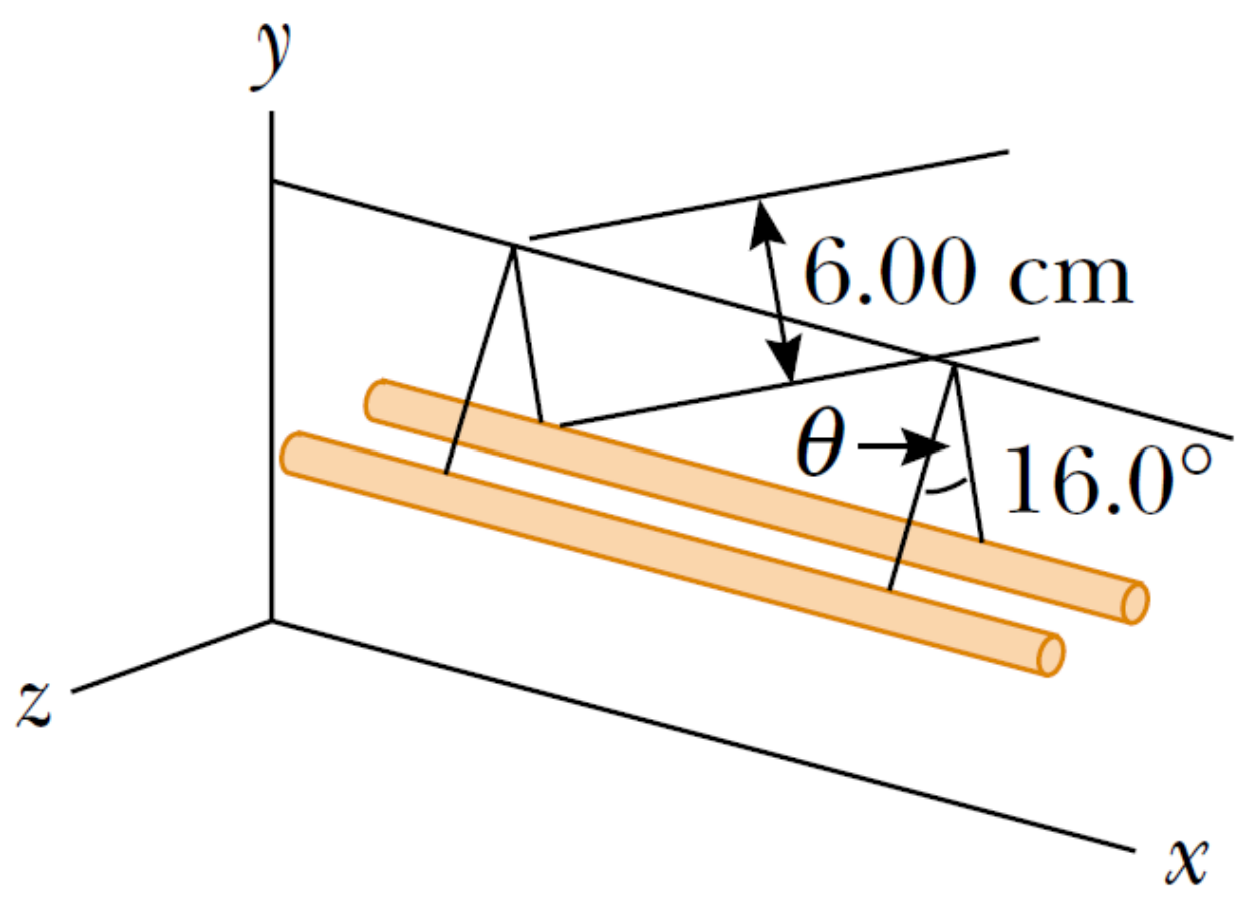
\includegraphics[width=6cm]{oz03/resources/oef-5-opgave.png}
    
%     \textbf{Figuur 3.3}
% \end{figure}

% \begin{description}[labelwidth=1.5cm, leftmargin=!]
%     \item[Geg. :]   $ \lambda_m = 40 $ g/m; $ l_{draad} = 6,00 $ cm; $ \theta = 16^{\circ} $;
% \end{description}

% \begin{figure}[H]
%     \centering
%     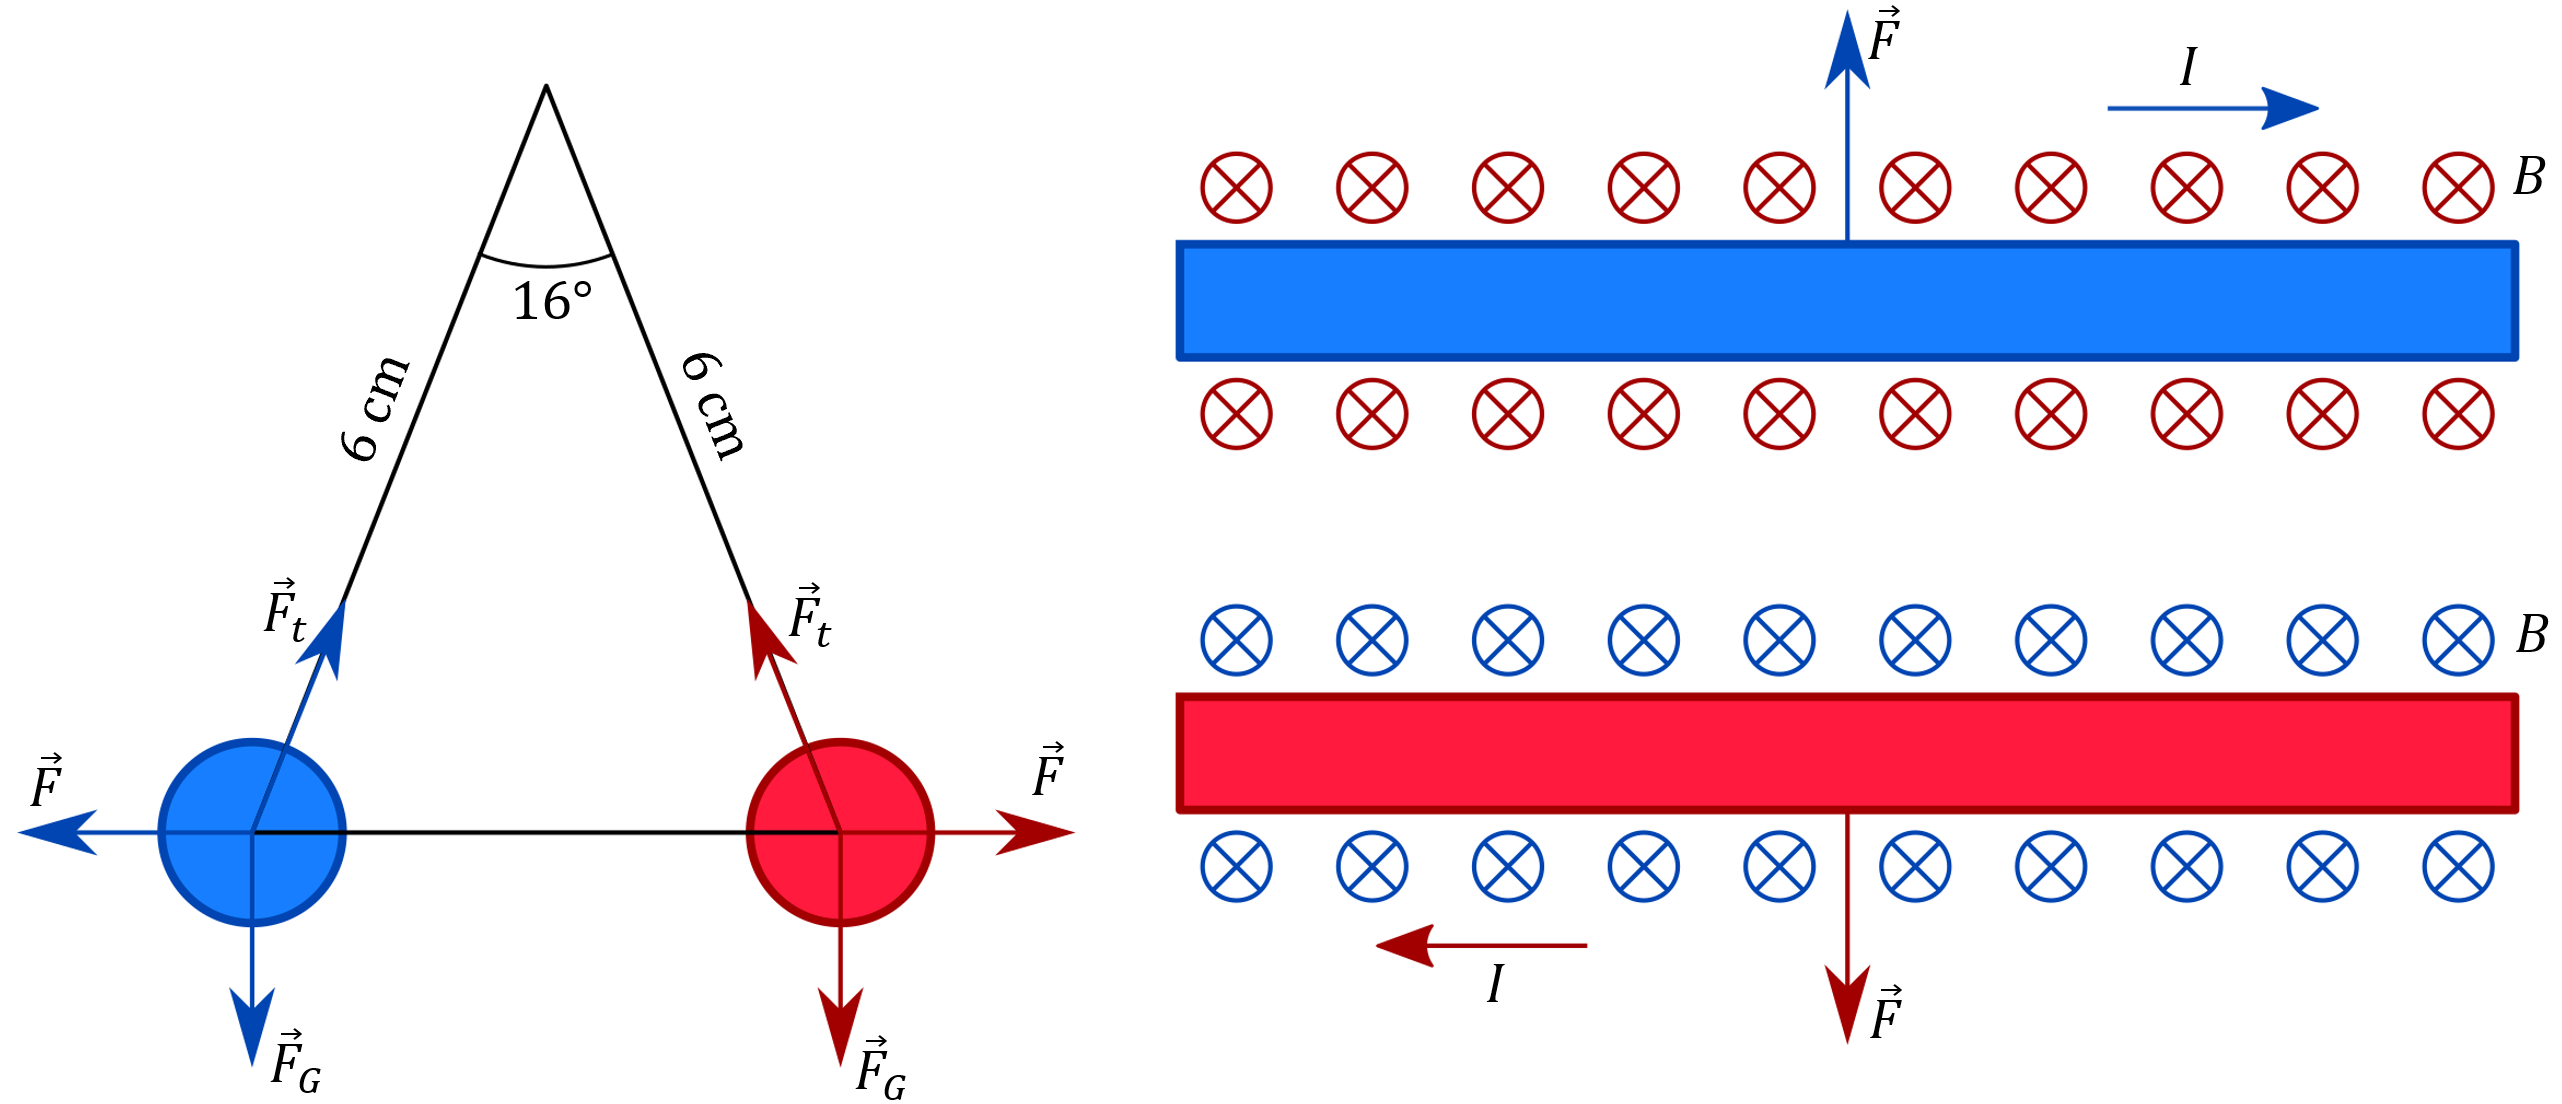
\includegraphics[width=12cm]{oz03/resources/oef-5-schets.png}
    
%     \textbf{Schets 3.2}
% \end{figure}

% \begin{enumerate}[(a)]
%     \item De stromen zijn in tegengestelde zin.
%     \item 
%         \begin{description}[labelwidth=1.5cm, leftmargin=!]
%             \item[Gevr. :]  $ I $;
%             \item[Opl. :]   $ \sum F_y = 0 $
            
%                             \hspace{-0.57cm} $ \Leftrightarrow 
%                             F_t \cdot \sin{82^{\circ}} - F_G = 0 $
            
%                             \hspace{-0.57cm} $ \Leftrightarrow 
%                             F_t = \dfrac{m \cdot g}{\sin{82^{\circ}}}
%                             = \dfrac{\lambda_m \cdot l \cdot g}{\sin{82^{\circ}}} $
                            
%                             \vspace{0.5cm}
                            
%                             $ \sum F_x = 0 $
            
%                             \hspace{-0.57cm} $ \Leftrightarrow 
%                             F_t \cdot \cos{82^{\circ}} - F = 0 $
            
%                             \hspace{-0.57cm} $ \Leftrightarrow 
%                             F = F_t \cdot \cos{82^{\circ}} 
%                             = \dfrac{\lambda_m \cdot l \cdot g}{\sin{82^{\circ}}} \cdot \cos{82^{\circ}} 
%                             = \dfrac{\lambda_m \cdot l \cdot g}{\tan{82^{\circ}}} $
                            
%                             \vspace{0.5cm}
                            
%                             $ B = \dfrac{\mu_0 I}{2 \pi a}
%                             = \dfrac{\mu_0 I}{2 \pi \cdot 2 \cdot l_{draad} \cdot \sin{\dfrac{16^{\circ}}{2}}}
%                             = \dfrac{\mu_0 I}{4 \pi \cdot l_{draad} \cdot \sin{8^{\circ}}} $
                            
%                             \vspace{0.5cm}
                            
%                             $ d\vec{F} = I d\vec{s} \times \vec{B} $
                            
%                             \hspace{-0.57cm} $ \Leftrightarrow
%                             dF = I ds B $ \hspace{3.5cm} $ (\theta = 90^{\circ} \Rightarrow \sin{\theta} = 1) $
                            
%                             \hspace{-0.57cm} $ \Leftrightarrow 
%                             \int_{0}^{F}{dF} = \int_{0}^{l}{I B ds} $
                            
%                             \hspace{-0.57cm} $ \Leftrightarrow 
%                             F = I B l $
                            
%                             \hspace{-0.57cm} $ \Leftrightarrow 
%                             I = \dfrac{F}{B l} 
%                             = \dfrac{4\pi \cdot l_{draad} \cdot \sin{8^{\circ}} \cdot \lambda_m \cdot l \cdot g}{\mu_0 \cdot I \cdot l \cdot \tan{82^{\circ}}} 
%                             = \dfrac{4\pi \cdot l_{draad} \cdot \sin{8^{\circ}} \cdot \lambda_m \cdot g}{\mu_0 \cdot I \cdot \tan{82^{\circ}}} $
                            
%                             \hspace{-0.57cm} $ \Leftrightarrow
%                             I = \sqrt{\dfrac{4\pi \cdot l_{draad} \cdot \sin{8^{\circ}} \cdot \lambda_m \cdot g}{\mu_0 \cdot \tan{82^{\circ}}}} 
%                             = \sqrt{\dfrac{4\pi \cdot 6,00 \cdot 10^{-2} \cdot \sin{8^{\circ}} \cdot 40 \cdot 10^{-3} \cdot 9,81}{4\pi \cdot 10^{-7} \cdot \tan{82^{\circ}}}} $ 
                            
%                             \hspace{0.17cm} $ = 67,86081 $ A 
%                             $ \approx 67,9 $ A
%         \end{description}
% \end{enumerate}

% \vspace{1cm}